\chapter{Ergebnisse}

\section{Interpretation}
\subsection{Transinformation}
Die Transinformation ist ein nützliches Werkzeug, um in einem komplexen Parameterraum eine erste Orientierung zu bekommen. Da wir es in diesem Kontext mit zwei distinkten Sätzen an Parametern zu tun haben, wurden drei Korrelationsmatrizen geplottet: eine welche die Transinformation zwischen TSI-Parametern betrachtet, eine weitere für die PSF-Parameter und eine für Korrelationen zwischen PSF- und TSI-Parametern.\\
Die TSI- und PSF-Korrelationsmatrizen haben auf beiden Achsen dieselben Parameter. Eine Konsequenz daraus ist, dass die Matrizen sowohl symmetrisch sind, als auch den Transinformationswert 1 auf der Diagonalen besitzen, da eine Verteilung mit sich selbst völlig korreliert (Abb. \ref{heatmap_tsi_inline} und \ref{heatmap_psf_inline}). Entsprechend weist die PSF/TSI Matrix keines dieser beiden Merkmale auf (Abb. \ref{heatmap_psf_tsi_inline}).\\
\vfill\,

\begin{figure}[H]
	\centering
	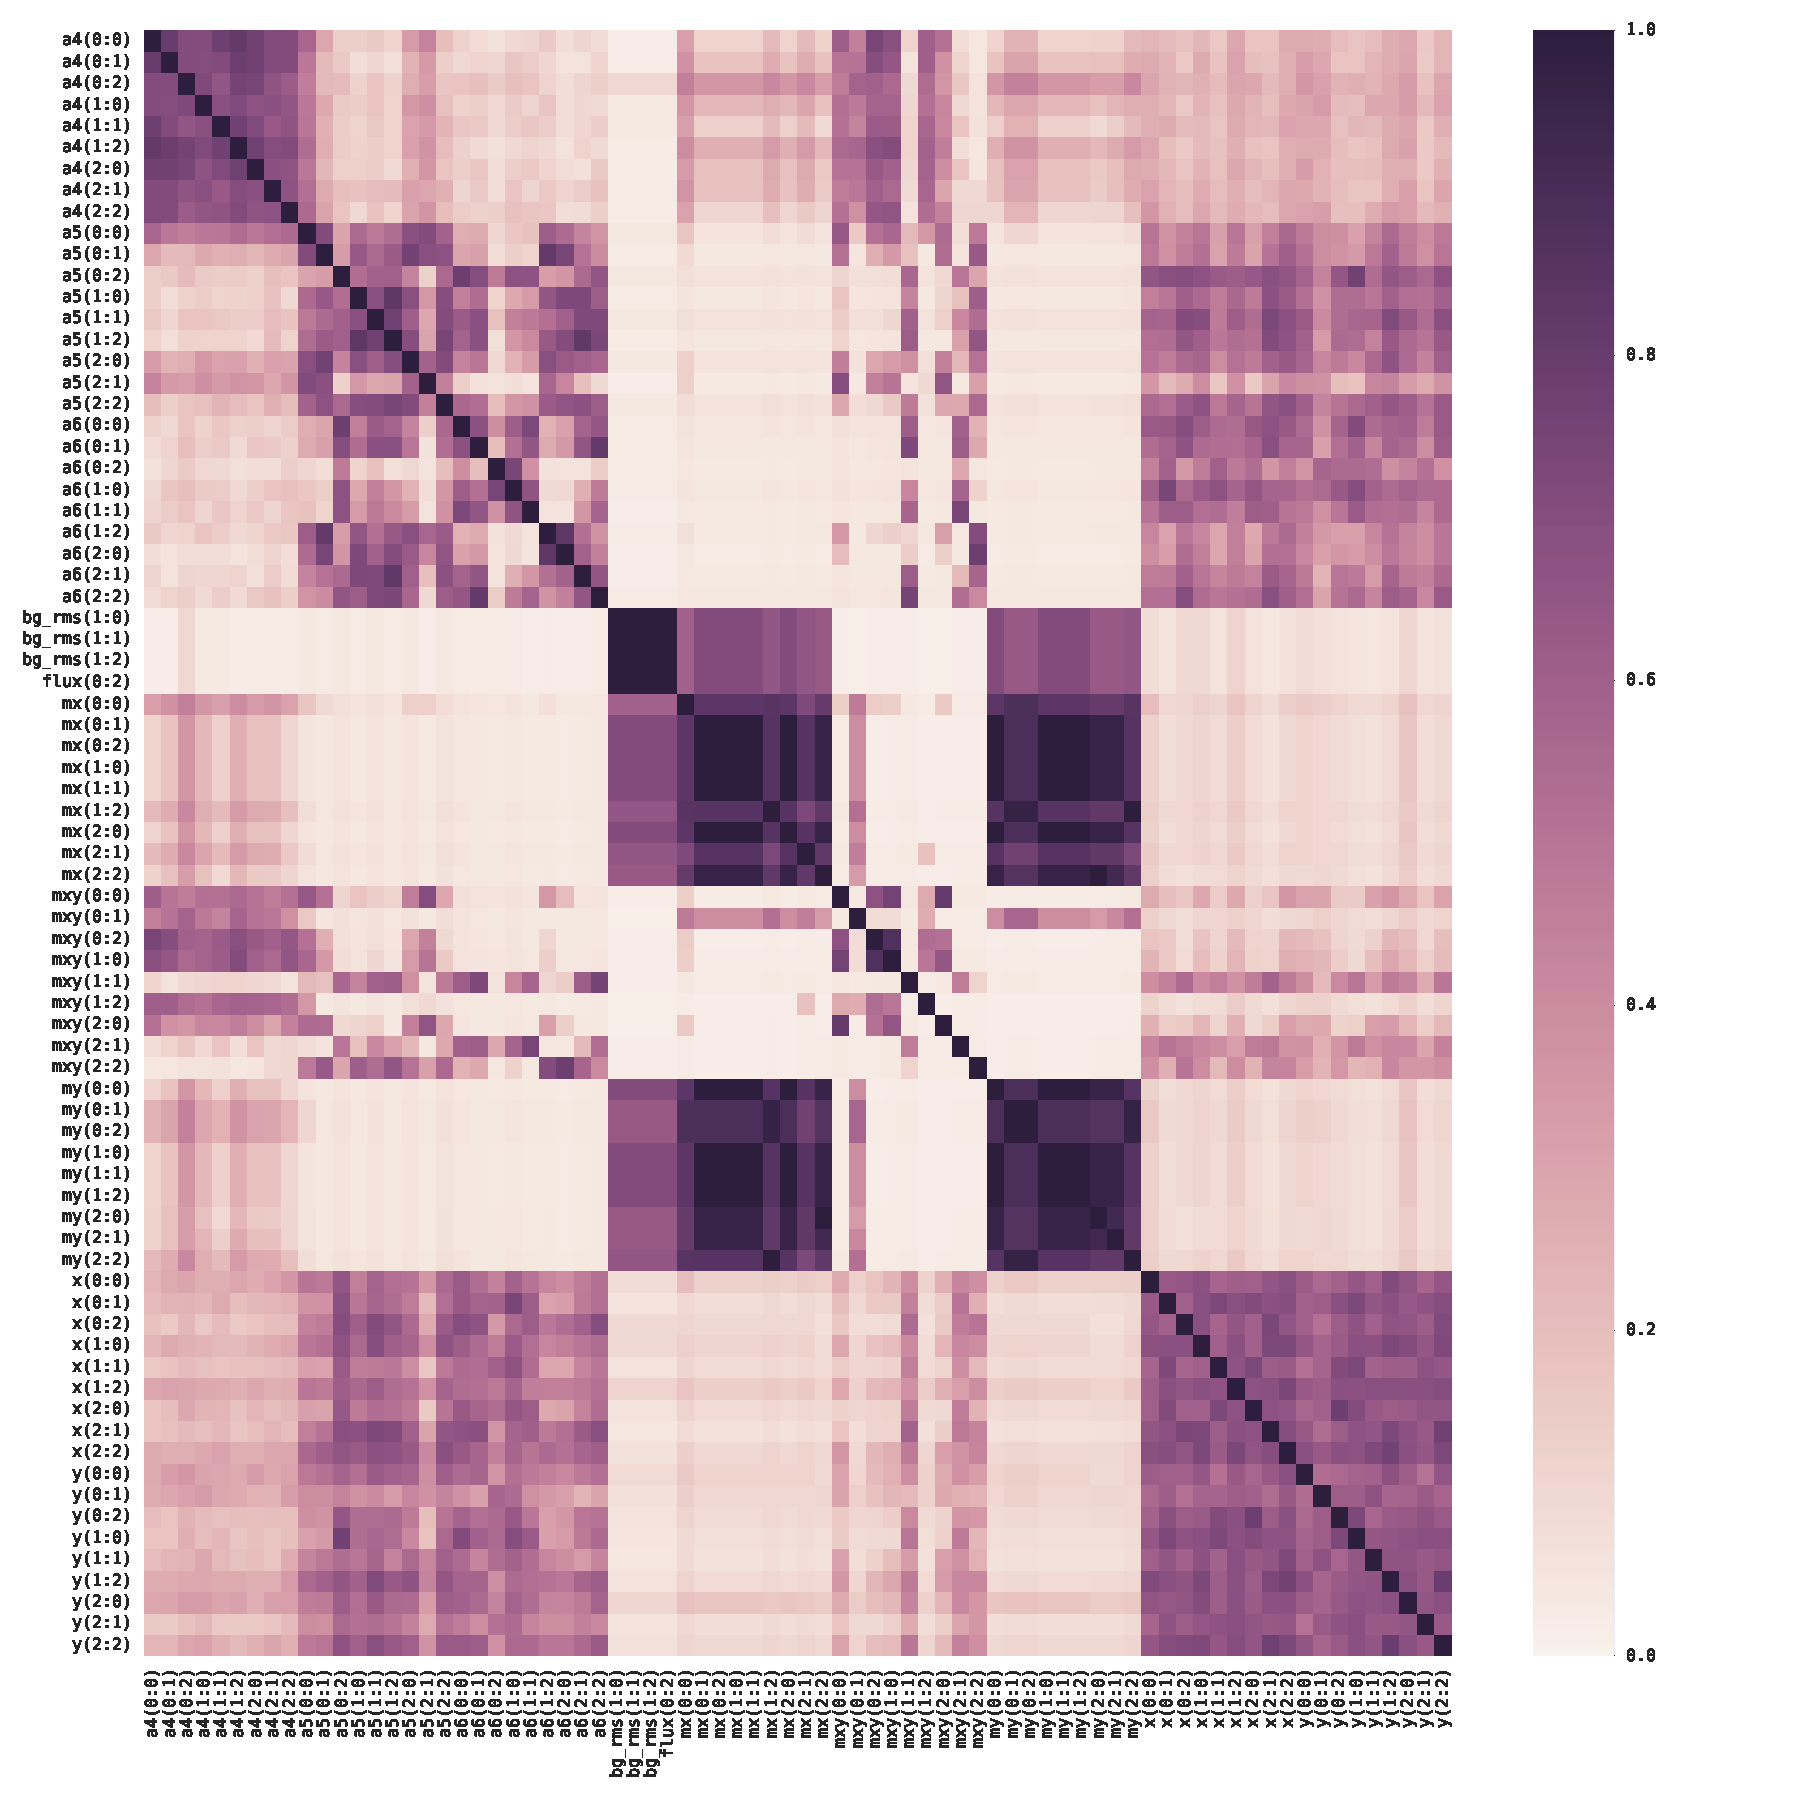
\includegraphics[scale=.56]{heatmaps/psf.pdf}
	\caption[Transinformations-Heatmap der PSF-Parameter]{Transinformations-Heatmap der PSF-Parameter. Jeder Pixel auf der Karte entspricht einem normierten Transinformations-Index. Die Achsen zeigen den Bezeichner des Parameters so wie seine Position innerhalb eines $3\times 3$-Gitters auf dem Sensor.  Da beide Achsen die selben Parameter enthalten nimmt jeder Wert auf der Diagonalen den Wert $\num{1}$ an.}
    \label{heatmap_psf_inline}
\end{figure}

\begin{figure}[H]
	\centering
	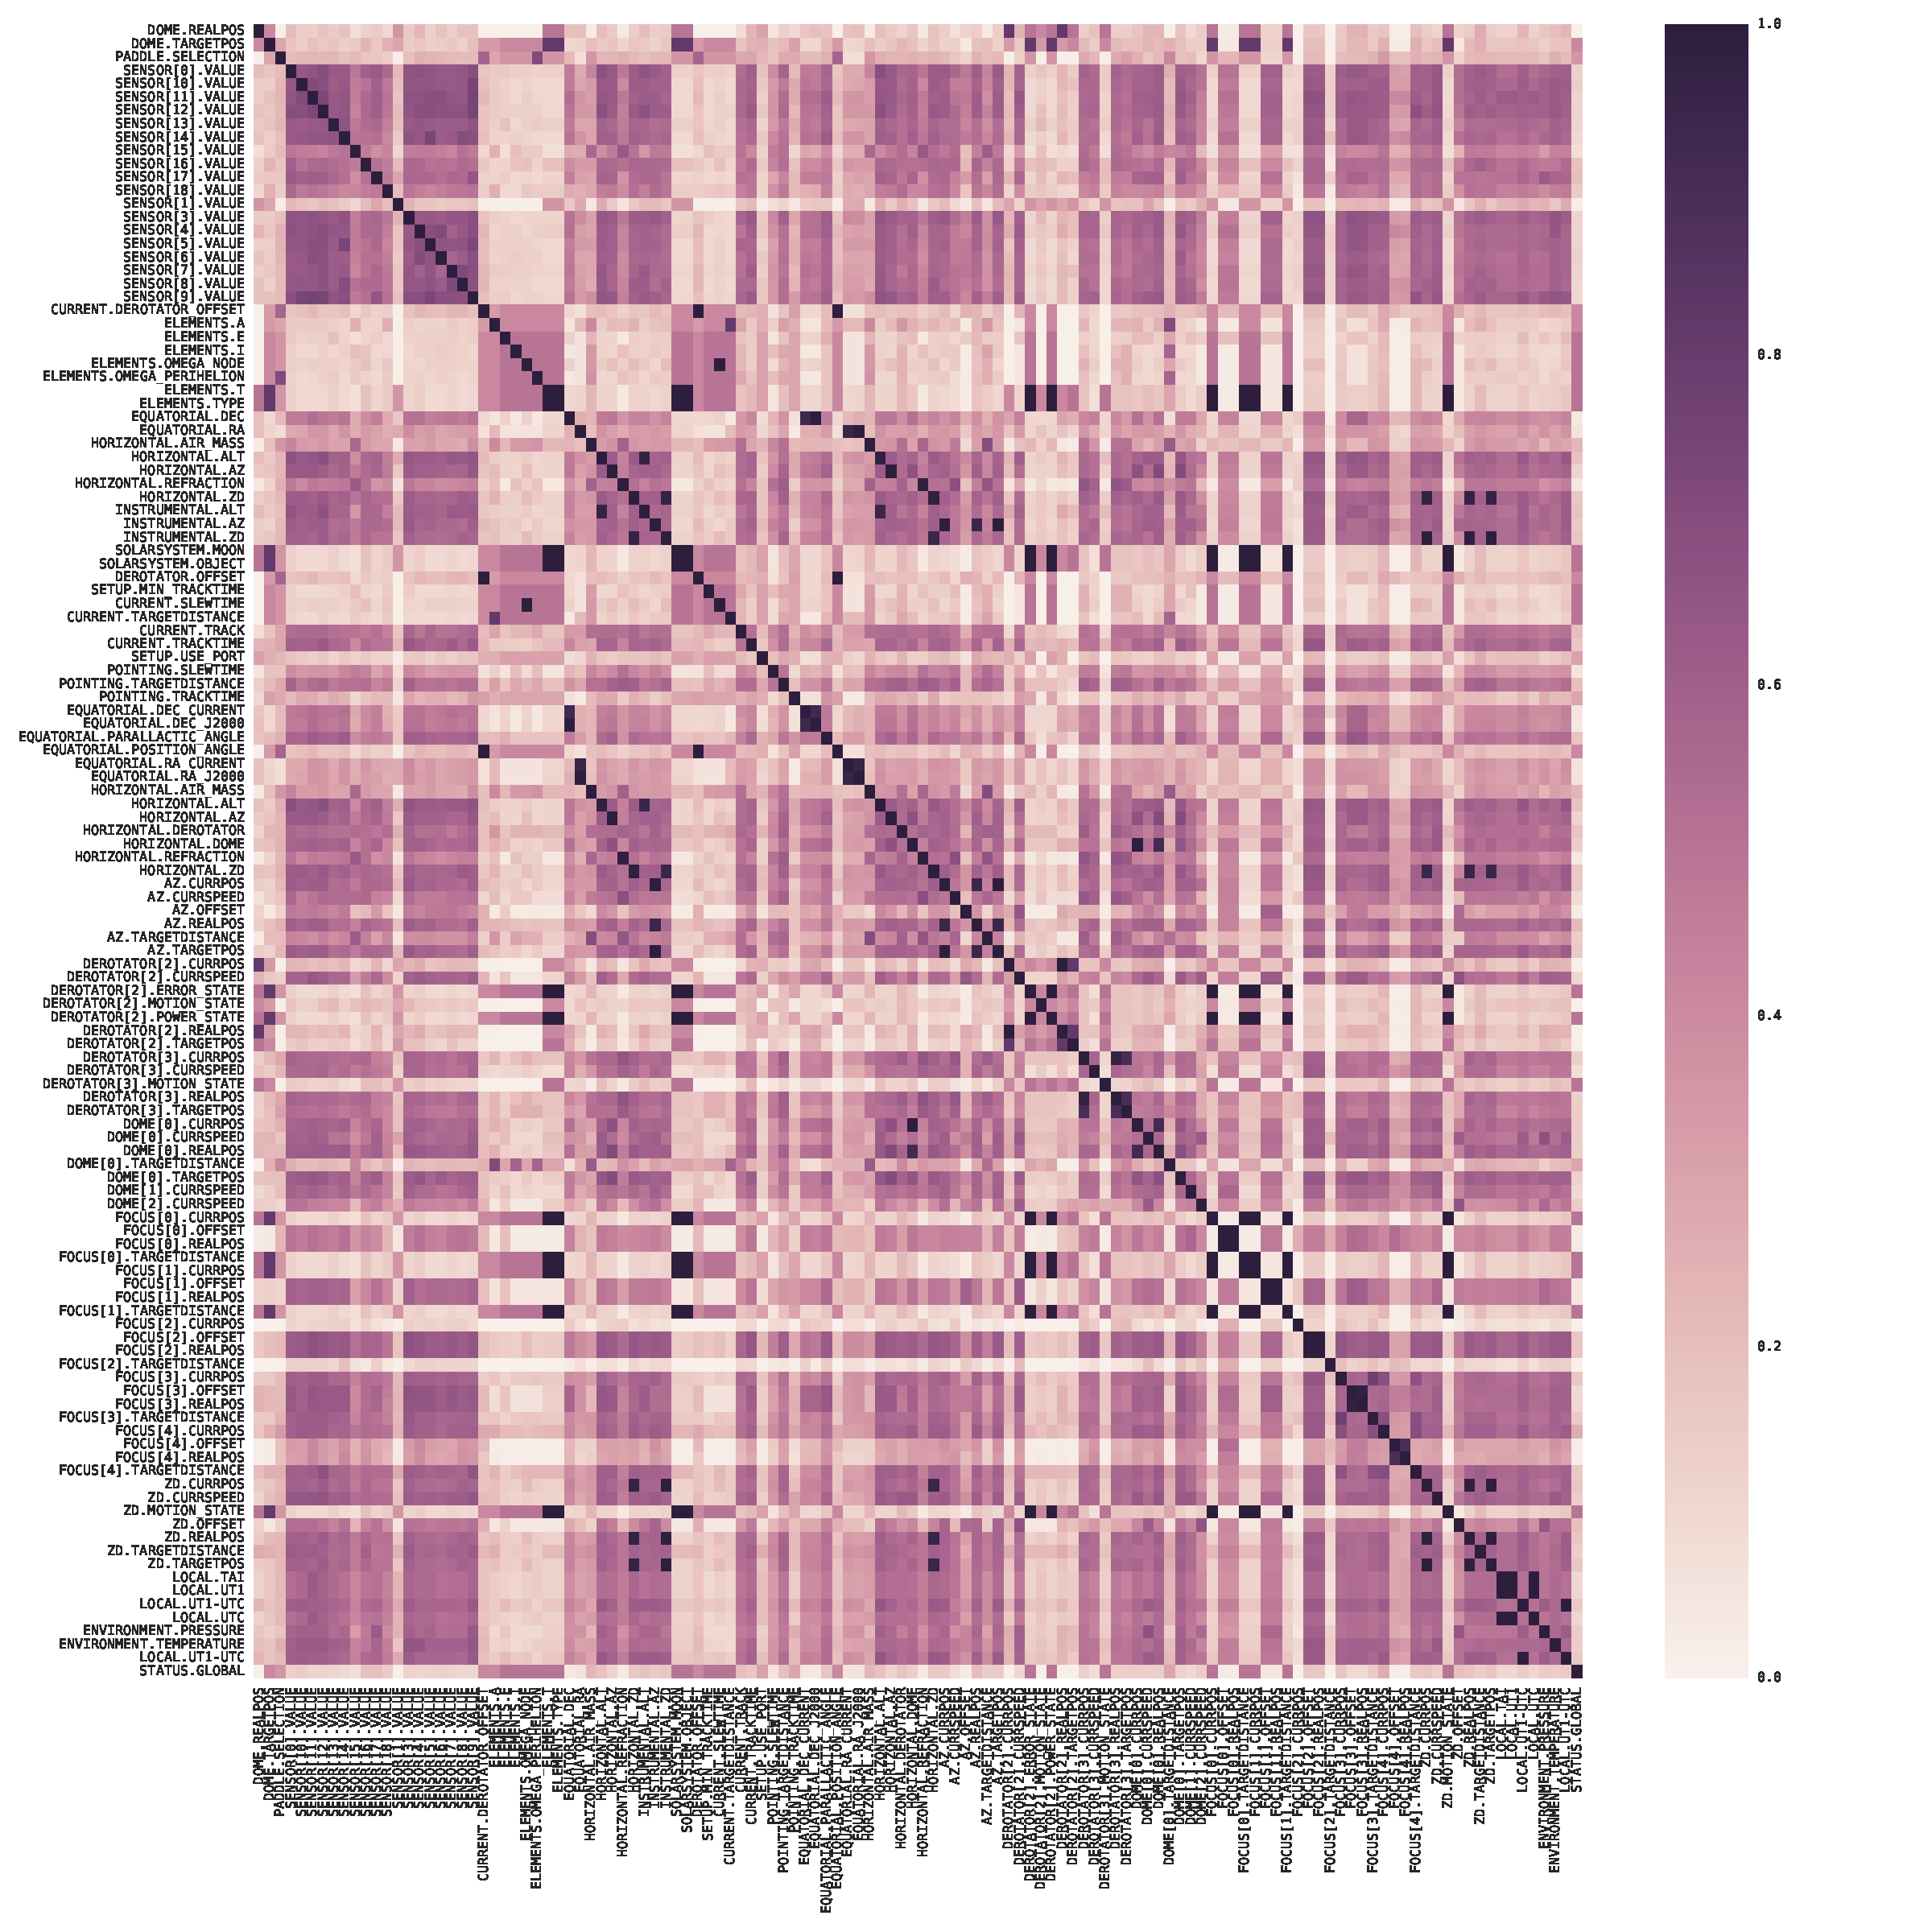
\includegraphics[scale=.42]{heatmaps/tsi.pdf}
	\caption[Transinformations-Heatmap der TSI-Parameter]{Transinformations-Heatmap der TSI-Parameter. Jeder Pixel auf der Karte entspricht einem normierten Transinformations-Index. Da beide Achsen die selben Parameter enthalten nimmt jeder Wert auf der Diagonalen den Wert $\num{1}$ an.}
    \label{heatmap_tsi_inline}
\end{figure}

\begin{figure}[H]
	\centering
	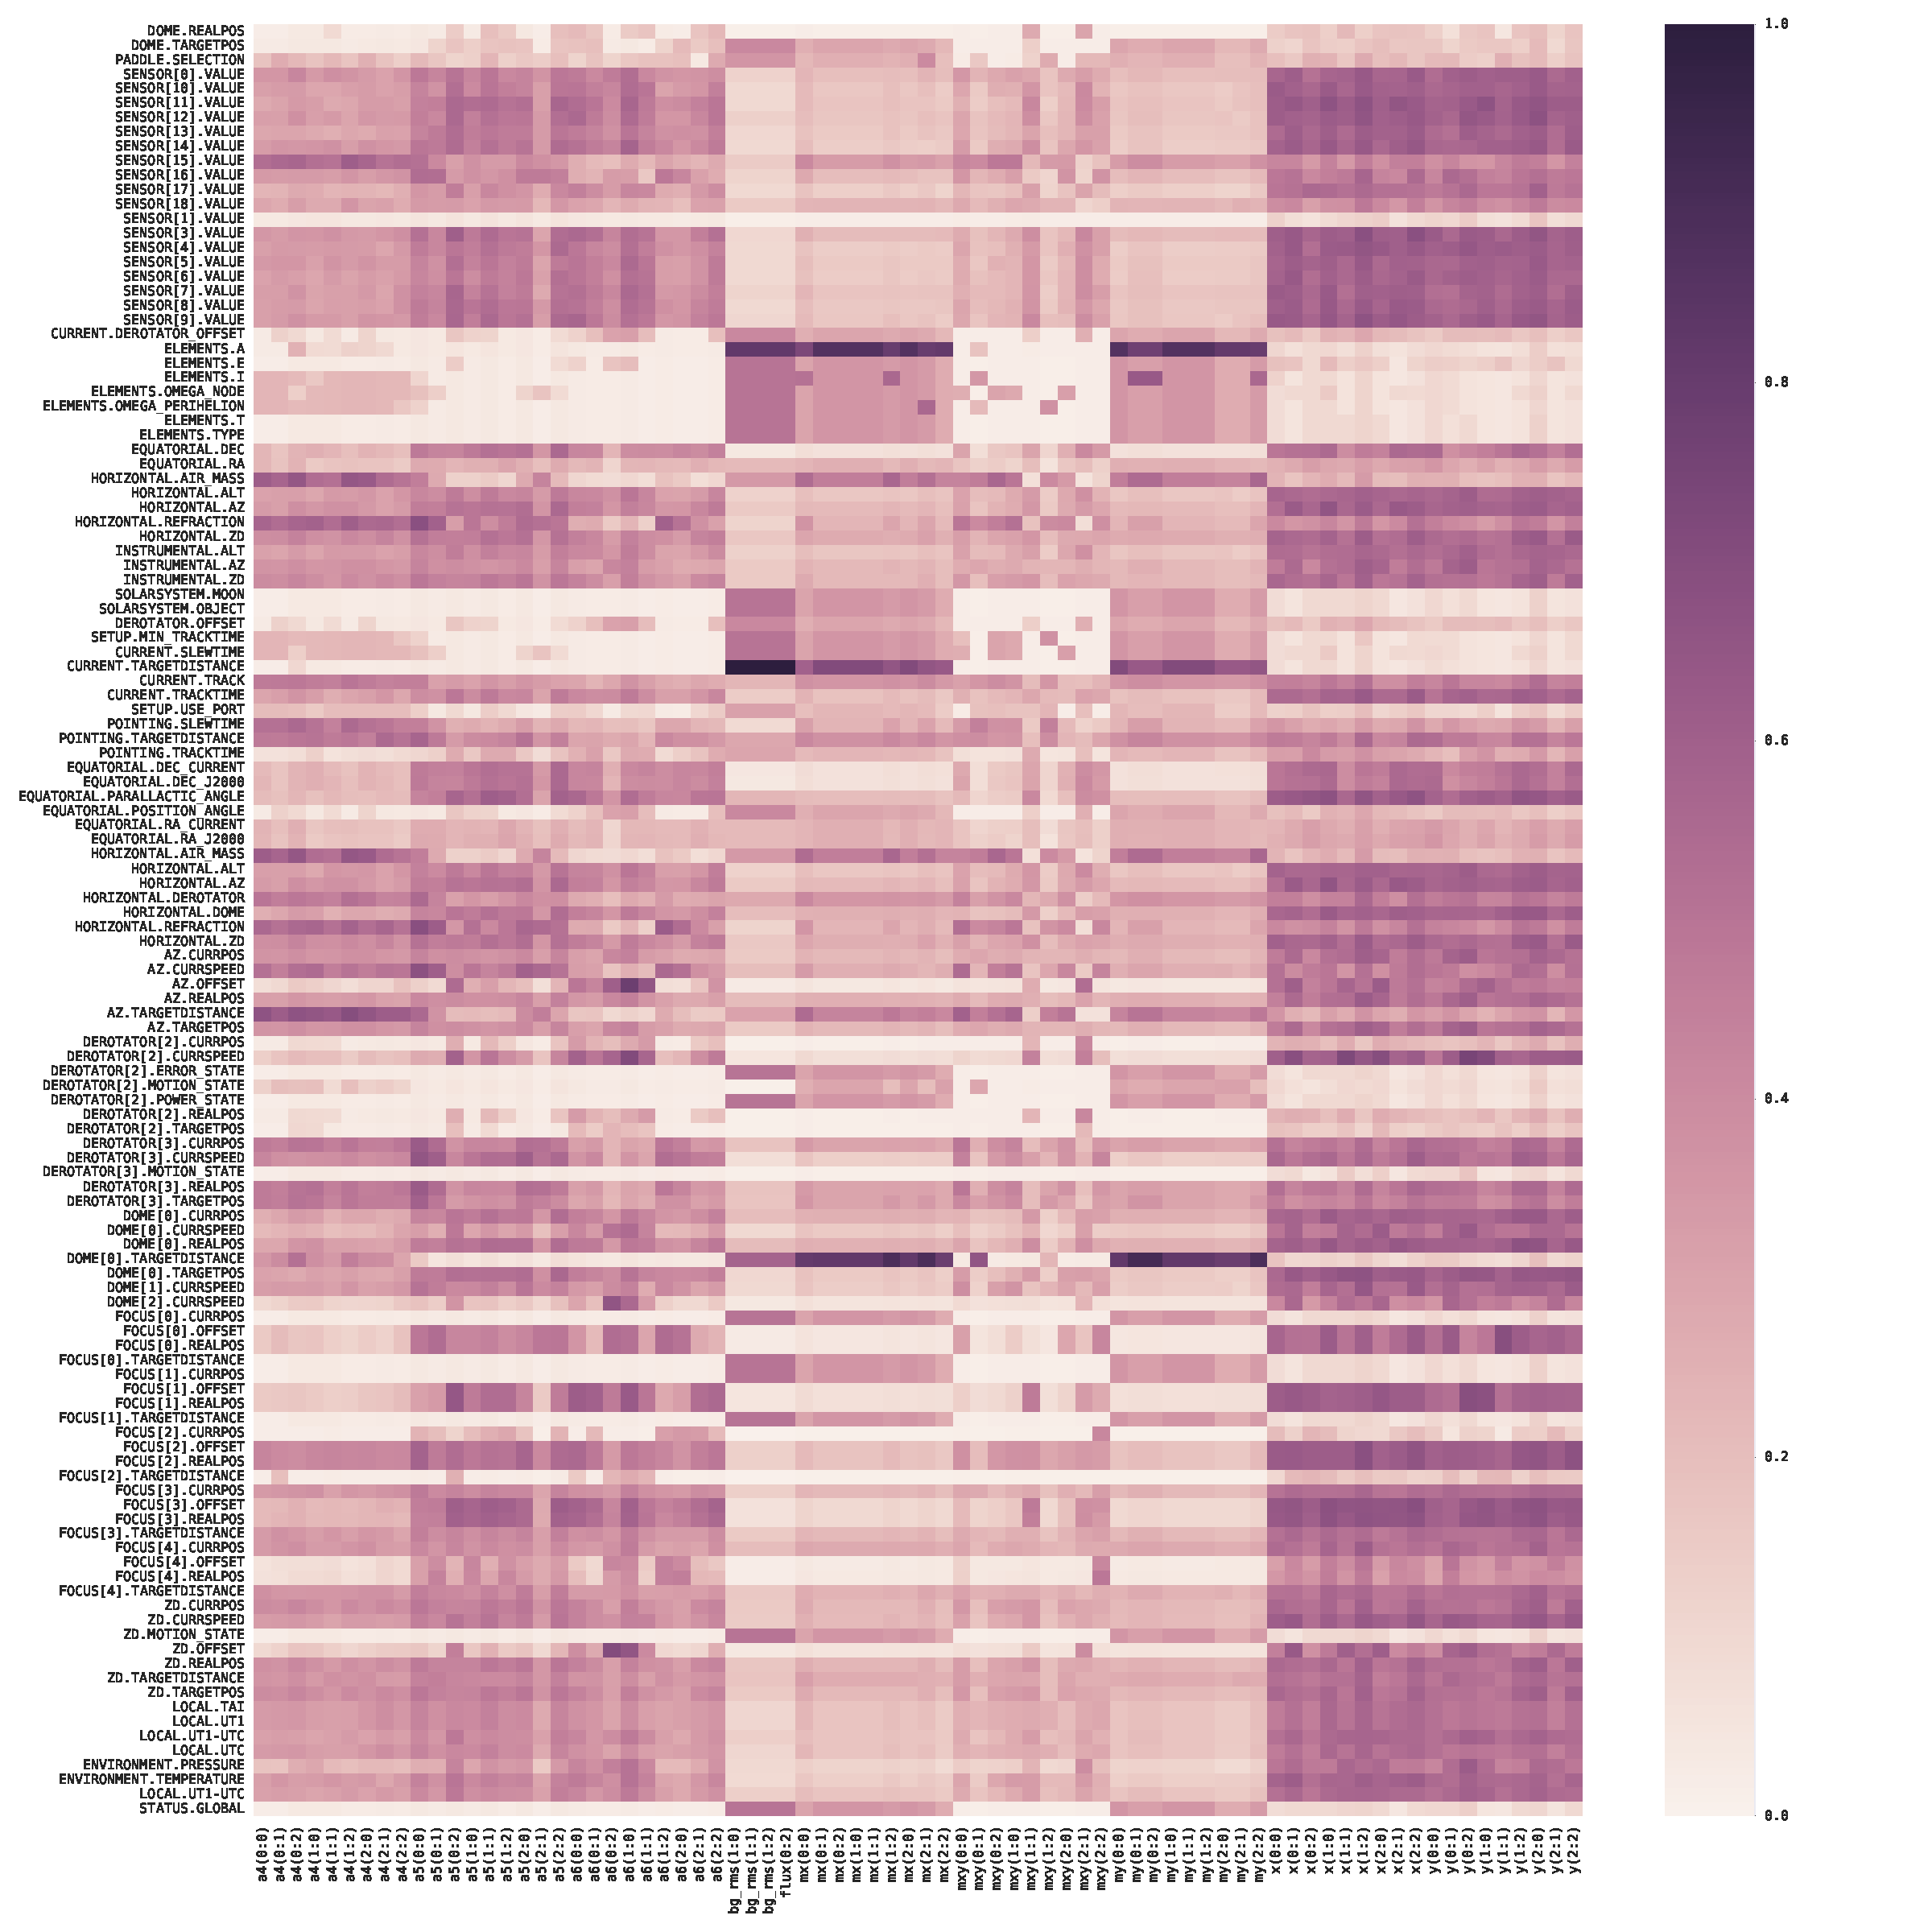
\includegraphics[scale=.42]{heatmaps/psf_tsi.pdf}
	\caption[Heatmap der Transinformation Korrelationsmatrix zwischen PSF- und TSI-Parametern]{Heatmap der Transinformation Korrelationsmatrix zwischen PSF- und TSI-Parametern. Jeder Pixel auf der Karte entspricht einem normierten Transinformations-Index.}
    \label{heatmap_psf_tsi_inline}
\end{figure}

Bei allen drei Matrizen fällt auf, dass sich Blöcke mit ähnlichen Transinformationswerten bilden. In erster Näherung kann dies durch die natürliche Gruppierung der Parameter auf den Achsen erklärt werden. Im Falle einer PSF-Achse wird jeder Parameter mehrfach aufgeführt (einmal für jeden Durchschnittswert im Gitter). Da sich die Position auf dem Detektor nur durch ein geringfügiges Rauschen äußert (vgl. \ref{psf_dists}) verhalten sich gleiche PSF-Parameter unterschiedlicher Gitterposition stochastisch sehr ähnlich. Bei einer TSI-Achse tauchen Parameter mit ähnlicher Verteilung auf, die aufgrund der alphabetischen Sortierung gruppiert werden. Oft sind dies Parameter und ihr Offset oder der selbe Parameter mit unterschiedlichem Namen. Beide Gruppierungen stochastisch ähnlicher Verteilungen auf den Achsen äußern sich in der geplotteten Matrix als Blöcke mit ähnlichem Wert.\\
Darüber hinaus gibt es hohe Korrelationswerte die kein bestimmtes Muster aufweisen und individuell betrachtet werden müssen. Besonders interessant sind Korrelationen mit der Position des Sekundärspiegels, da diese auf weitere Abhängigkeiten hinweisen könnten, welche in der Fokusfunktion zu berücksichtigen sind. Das die Transinformation ein guter Anhaltspunkt ist, bestätigen auch die bekannten Relationen. So wird die Sekundärspiegelposition mit Werten von $\sim\num{0.7}$ in der Korrelationsmatrix deutlich mit Temperatursensoren und Elevationsparametern korreliert.

\begin{figure}[H]
	\centering
	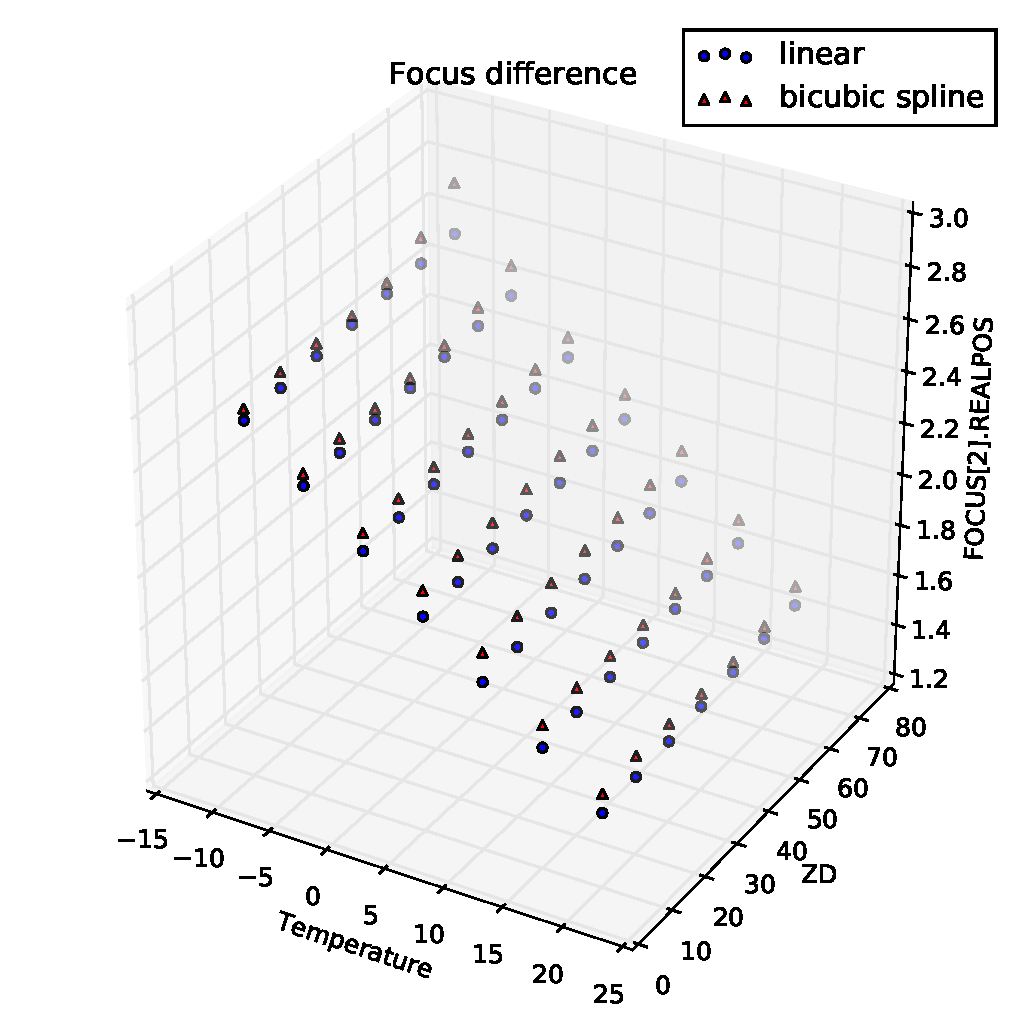
\includegraphics[scale=.6]{diff.pdf}
	\caption[Sekundärspiegelposition der linearen und bikubischen Näherung]{Sekundärspiegelposition der linearen und bikubischen Näherung. Es werden die absoluten Sekundärspiegelpositionen der beiden Fokusfunktionen für ausgewählte Punkte in Abhängigkeit von Temperatur und Elevation dargestellt.}
    \label{focus_surf}
\end{figure}

\subsection{Fokusfunktion}
Die Fokusfunktion wie sie momentan im Fraunhofer Teleskop Anwendung findet, justiert den Sekundärspiegel nur entlang der optischen Achse. Es wird folglich nur der Defokus berücksichtigt -- eine etwaige Berücksichtigung oder Korrektur des Astigmatismus erfolgt nicht. Der entsprechende Aberrations-Koeffizient ist $A_4$.\\
Eine Betrachtung von $A_4$ zeigt, dass die Median-Werte für hohe Temperaturen bei mittlerer Elevation stark zunehmen (Abb. \ref{psf_surf_a4_med_inline}). Im Allgemeinen streut $A_4$ eher stark, insbesondere bei hohen Temperaturen (Abb. \ref{psf_surf_a4_std_inline}). Bei diesen Plots wurden nur die als Beste ausgewählten Aufnahmen der jeweiligen Fokusserie verwendet.\\
Um auszuschließen, dass Seeing für die schlechten $A_4$ Werte bei hohen Temperaturen verantwortlich ist, kann die Windgeschwindigkeit und Windrichtung herangezogen werden. Die Verteilung hoher $A_4$ Werte im Polarplot zeigt keine ausgezeichneten Muster auf (Abb. \ref{wind_a4_inline}). Insbesondere sind für hohe Windgeschwindigkeiten aus südlicher Richtung (\enquote{Föhn}) keine schlechten $A_4$ Werte festzustellen. Insgesamt ist es somit naheliegend, dass weniger das Wetter als der durch die Temperatur auf das System ausgeübte Stress für den Defokus der Aufnahmen verantwortlich ist.\\

\begin{figure}[H]
	\centering
	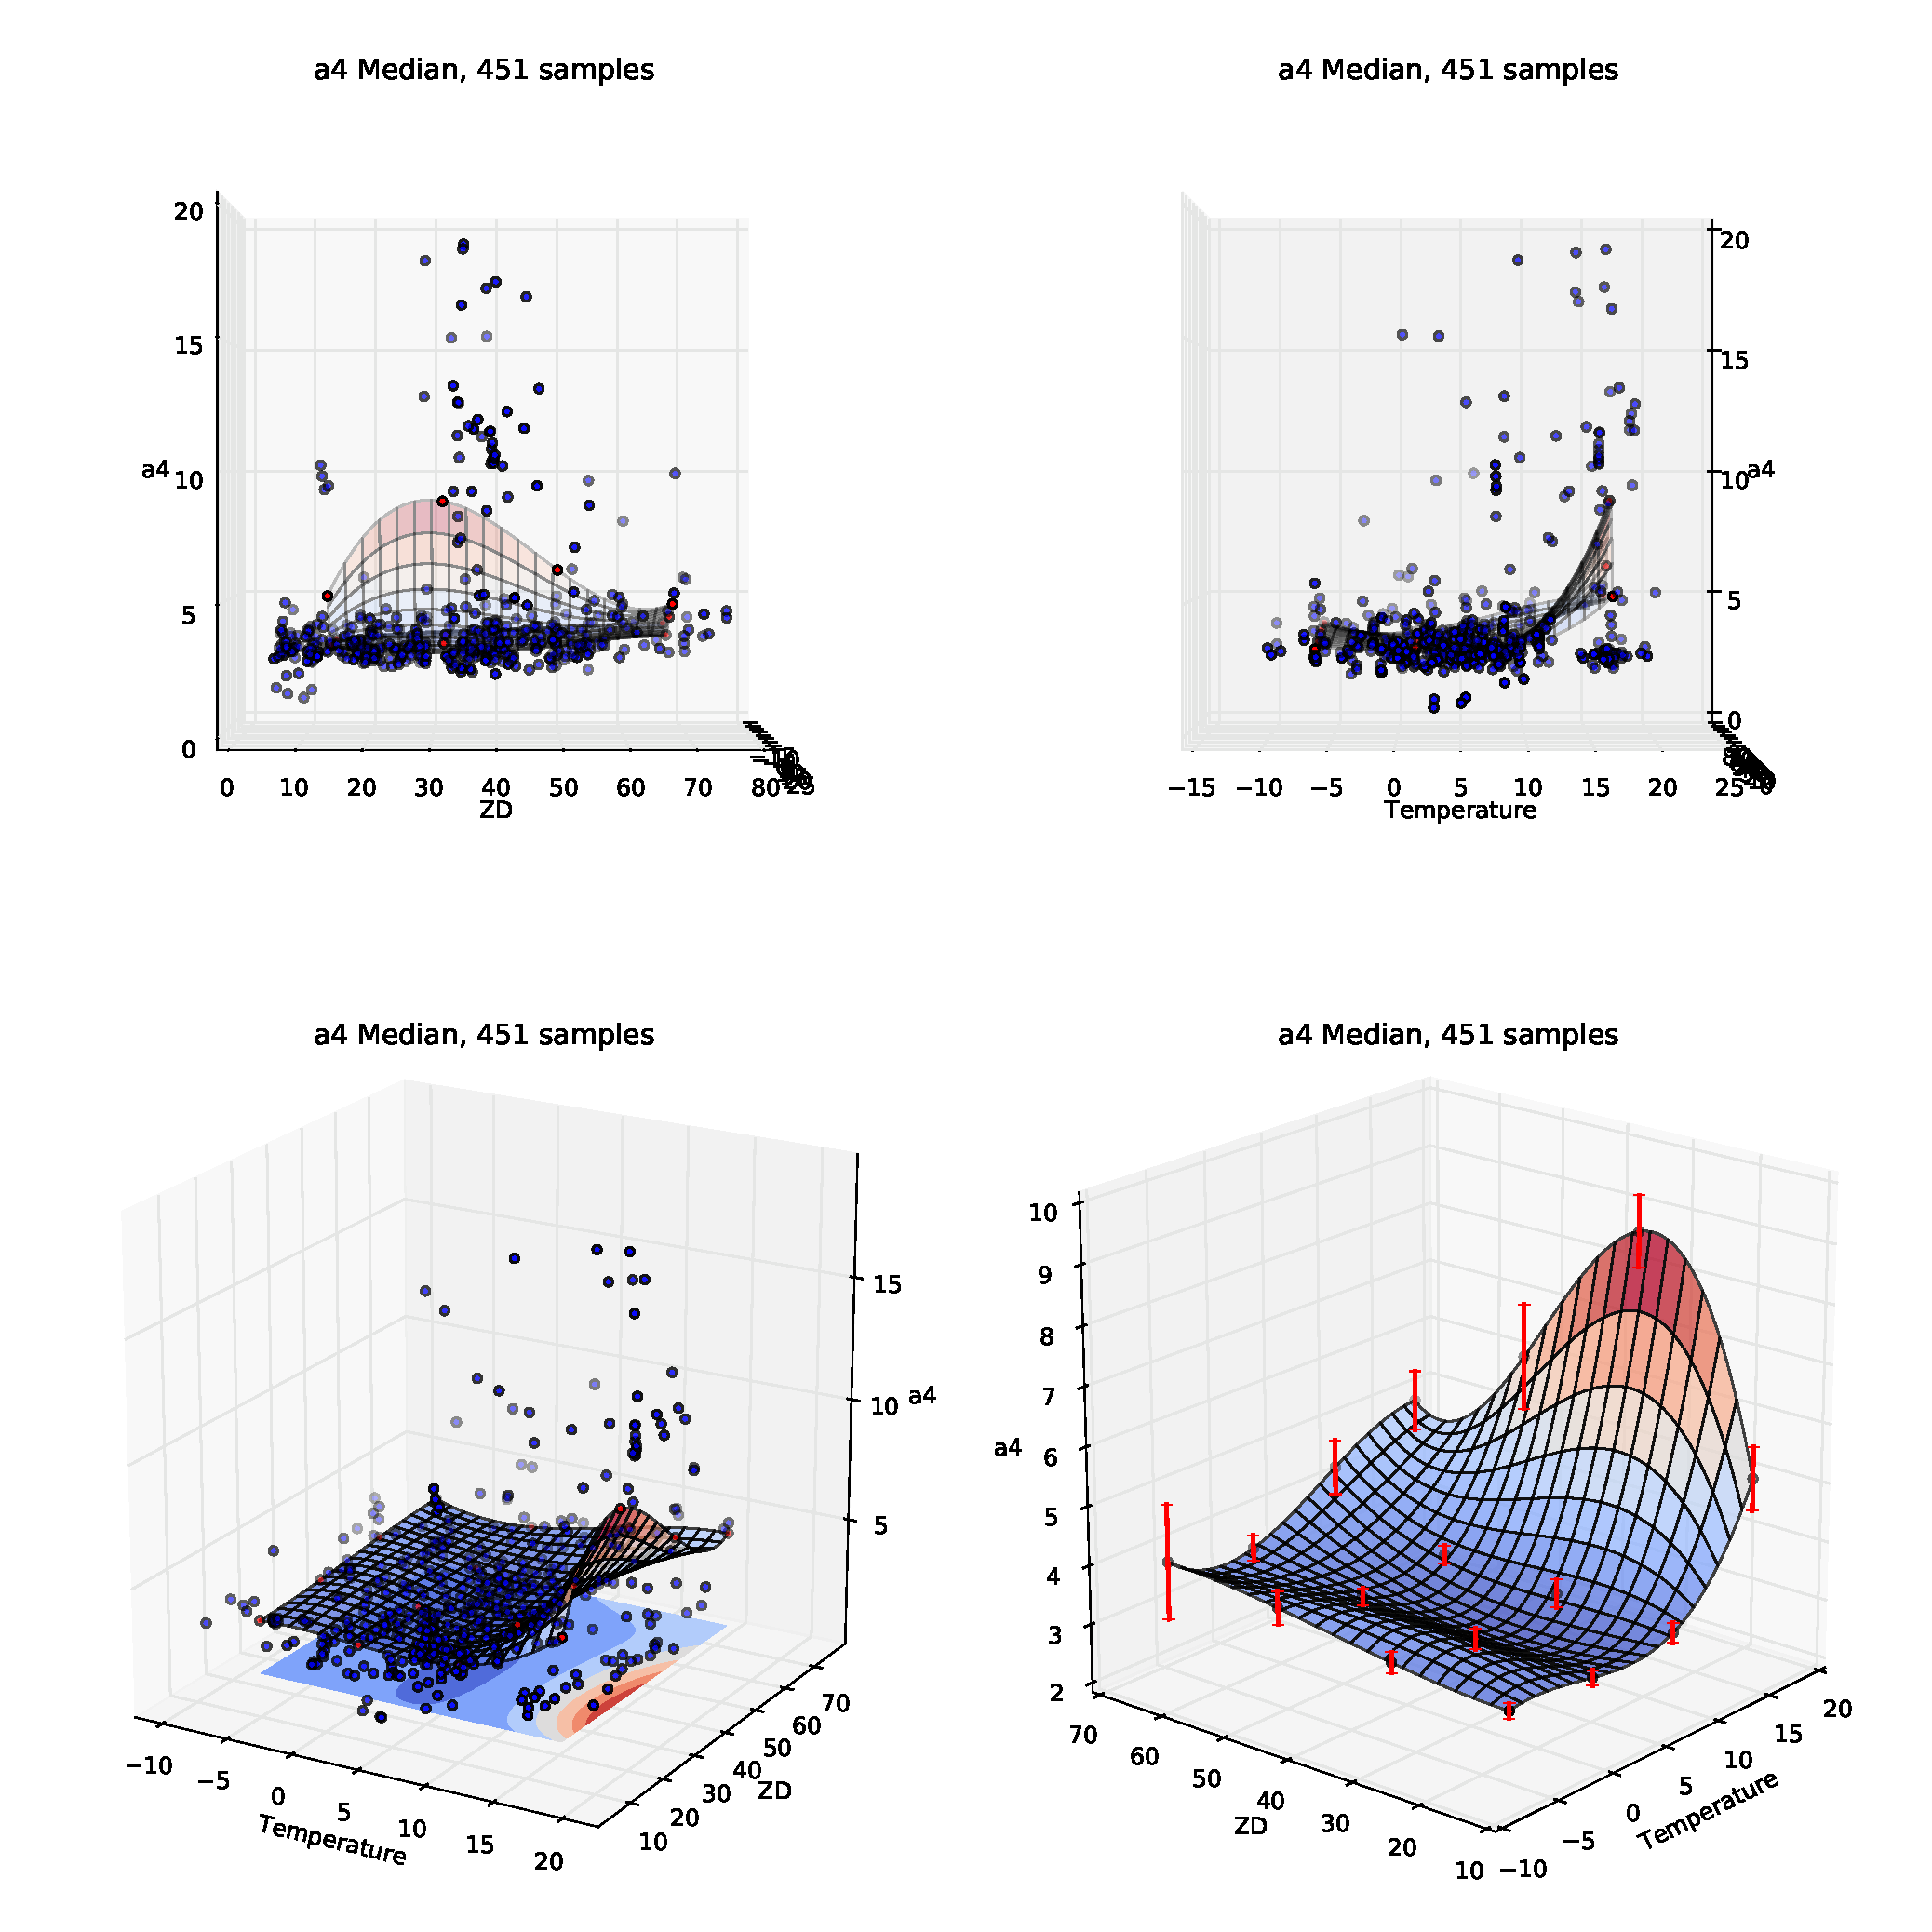
\includegraphics[scale=.48]{psf_surf/a4_med.pdf}
	\caption[Median Temperatur- und Elevationsabhängigkeit von $A_4$]{Median Temperatur- und Elevationsabhängigkeit von $A_4$. Es liegen 451 Fokusaufnahmen zugrunde, die jeweils einem blauen Punkt entsprechen. Die Plots oben links und rechts entsprechen der Projektion auf die Temperatur- und Elevations-Achse respektive. Die roten Kontrollpunkt wurden als Durchschnittswerte berechnet (mean). Die roten Balken an den Kontrollpunkten im Plot unten rechts sind ein Maß für die Streuung des Kontrollpunktes. }
    \label{psf_surf_a4_med_inline}
\end{figure}
\begin{figure}[H]
	\centering
	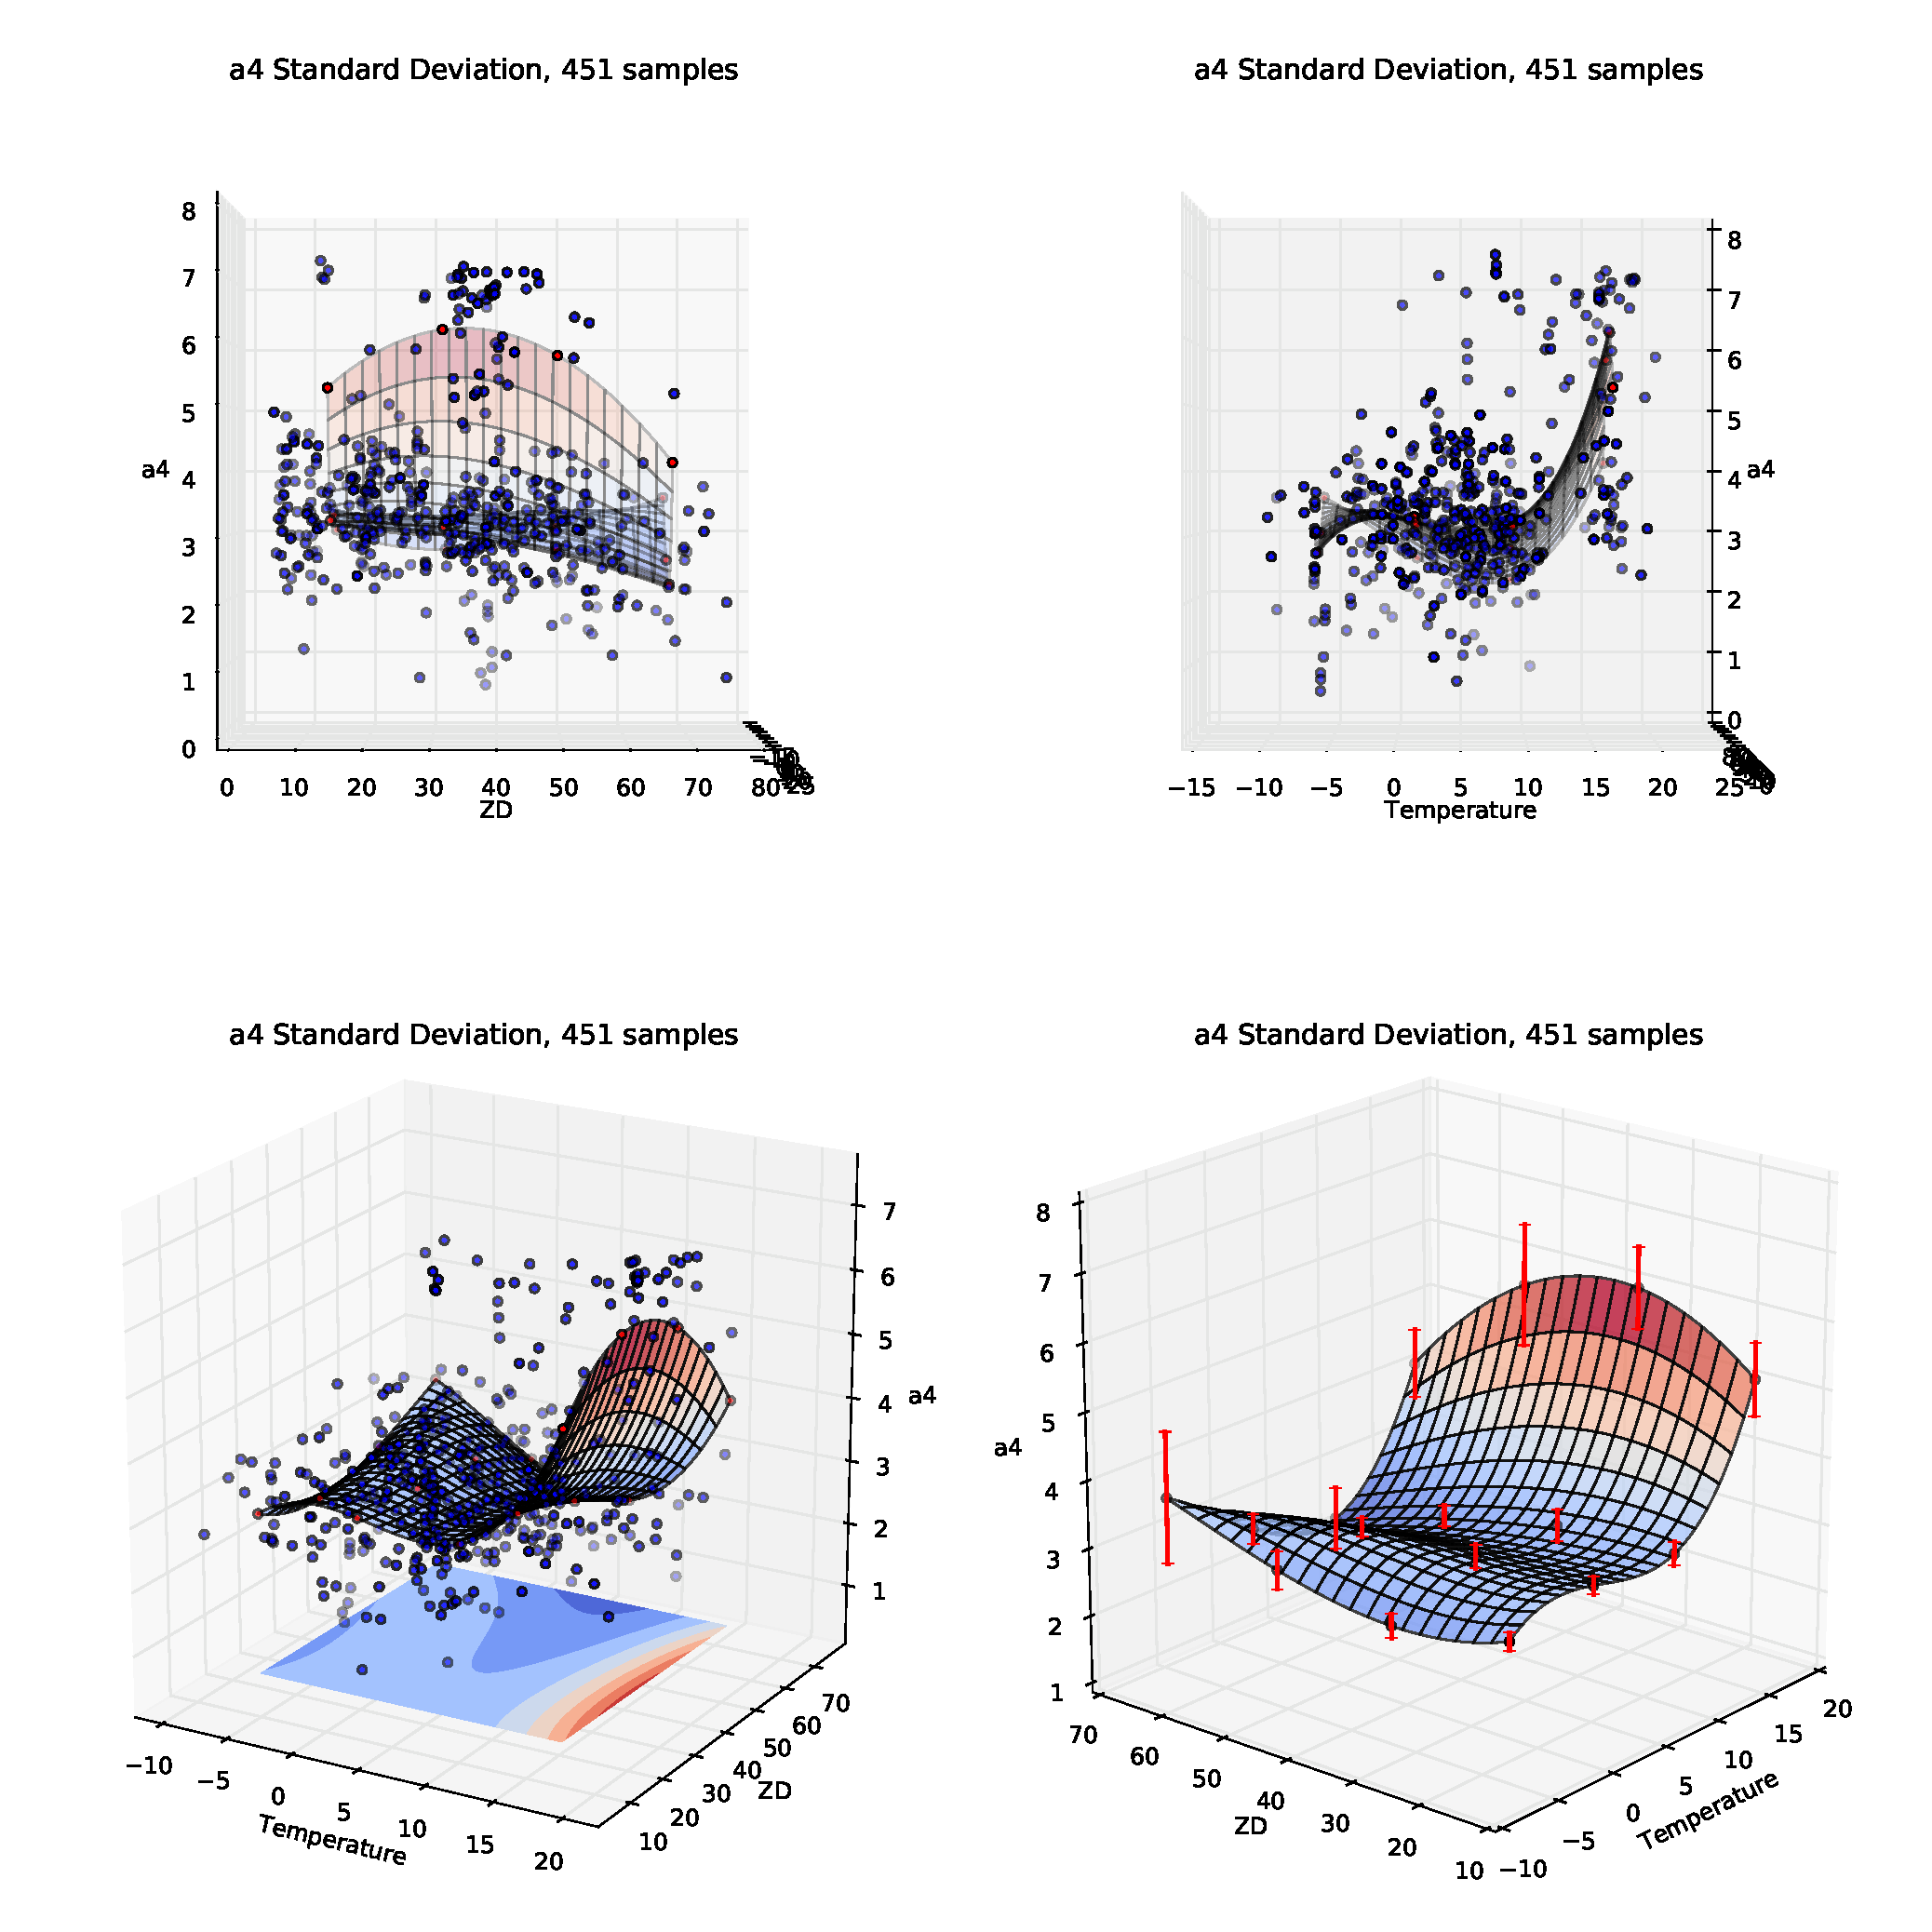
\includegraphics[scale=.48]{psf_surf/a4_std.pdf}
	\caption[Standardabweichung Temperatur- und Elevationsabhängigkeit von $A_4$]{Standardabweichung Temperatur- und Elevationsabhängigkeit von $A_4$. Es liegen 451 Fokusaufnahmen zugrunde, die jeweils einem blauen Punkt entsprechen. Die Plots oben links und rechts entsprechen der Projektion auf die Temperatur- und Elevations-Achse respektive. Die roten Kontrollpunkt wurden als Durchschnittswerte berechnet (mean). Die roten Balken an den Kontrollpunkten im Plot unten rechts sind ein Maß für die Streuung des Kontrollpunktes. }
    \label{psf_surf_a4_std_inline}
\end{figure}
\begin{figure}[H]
	\centering
	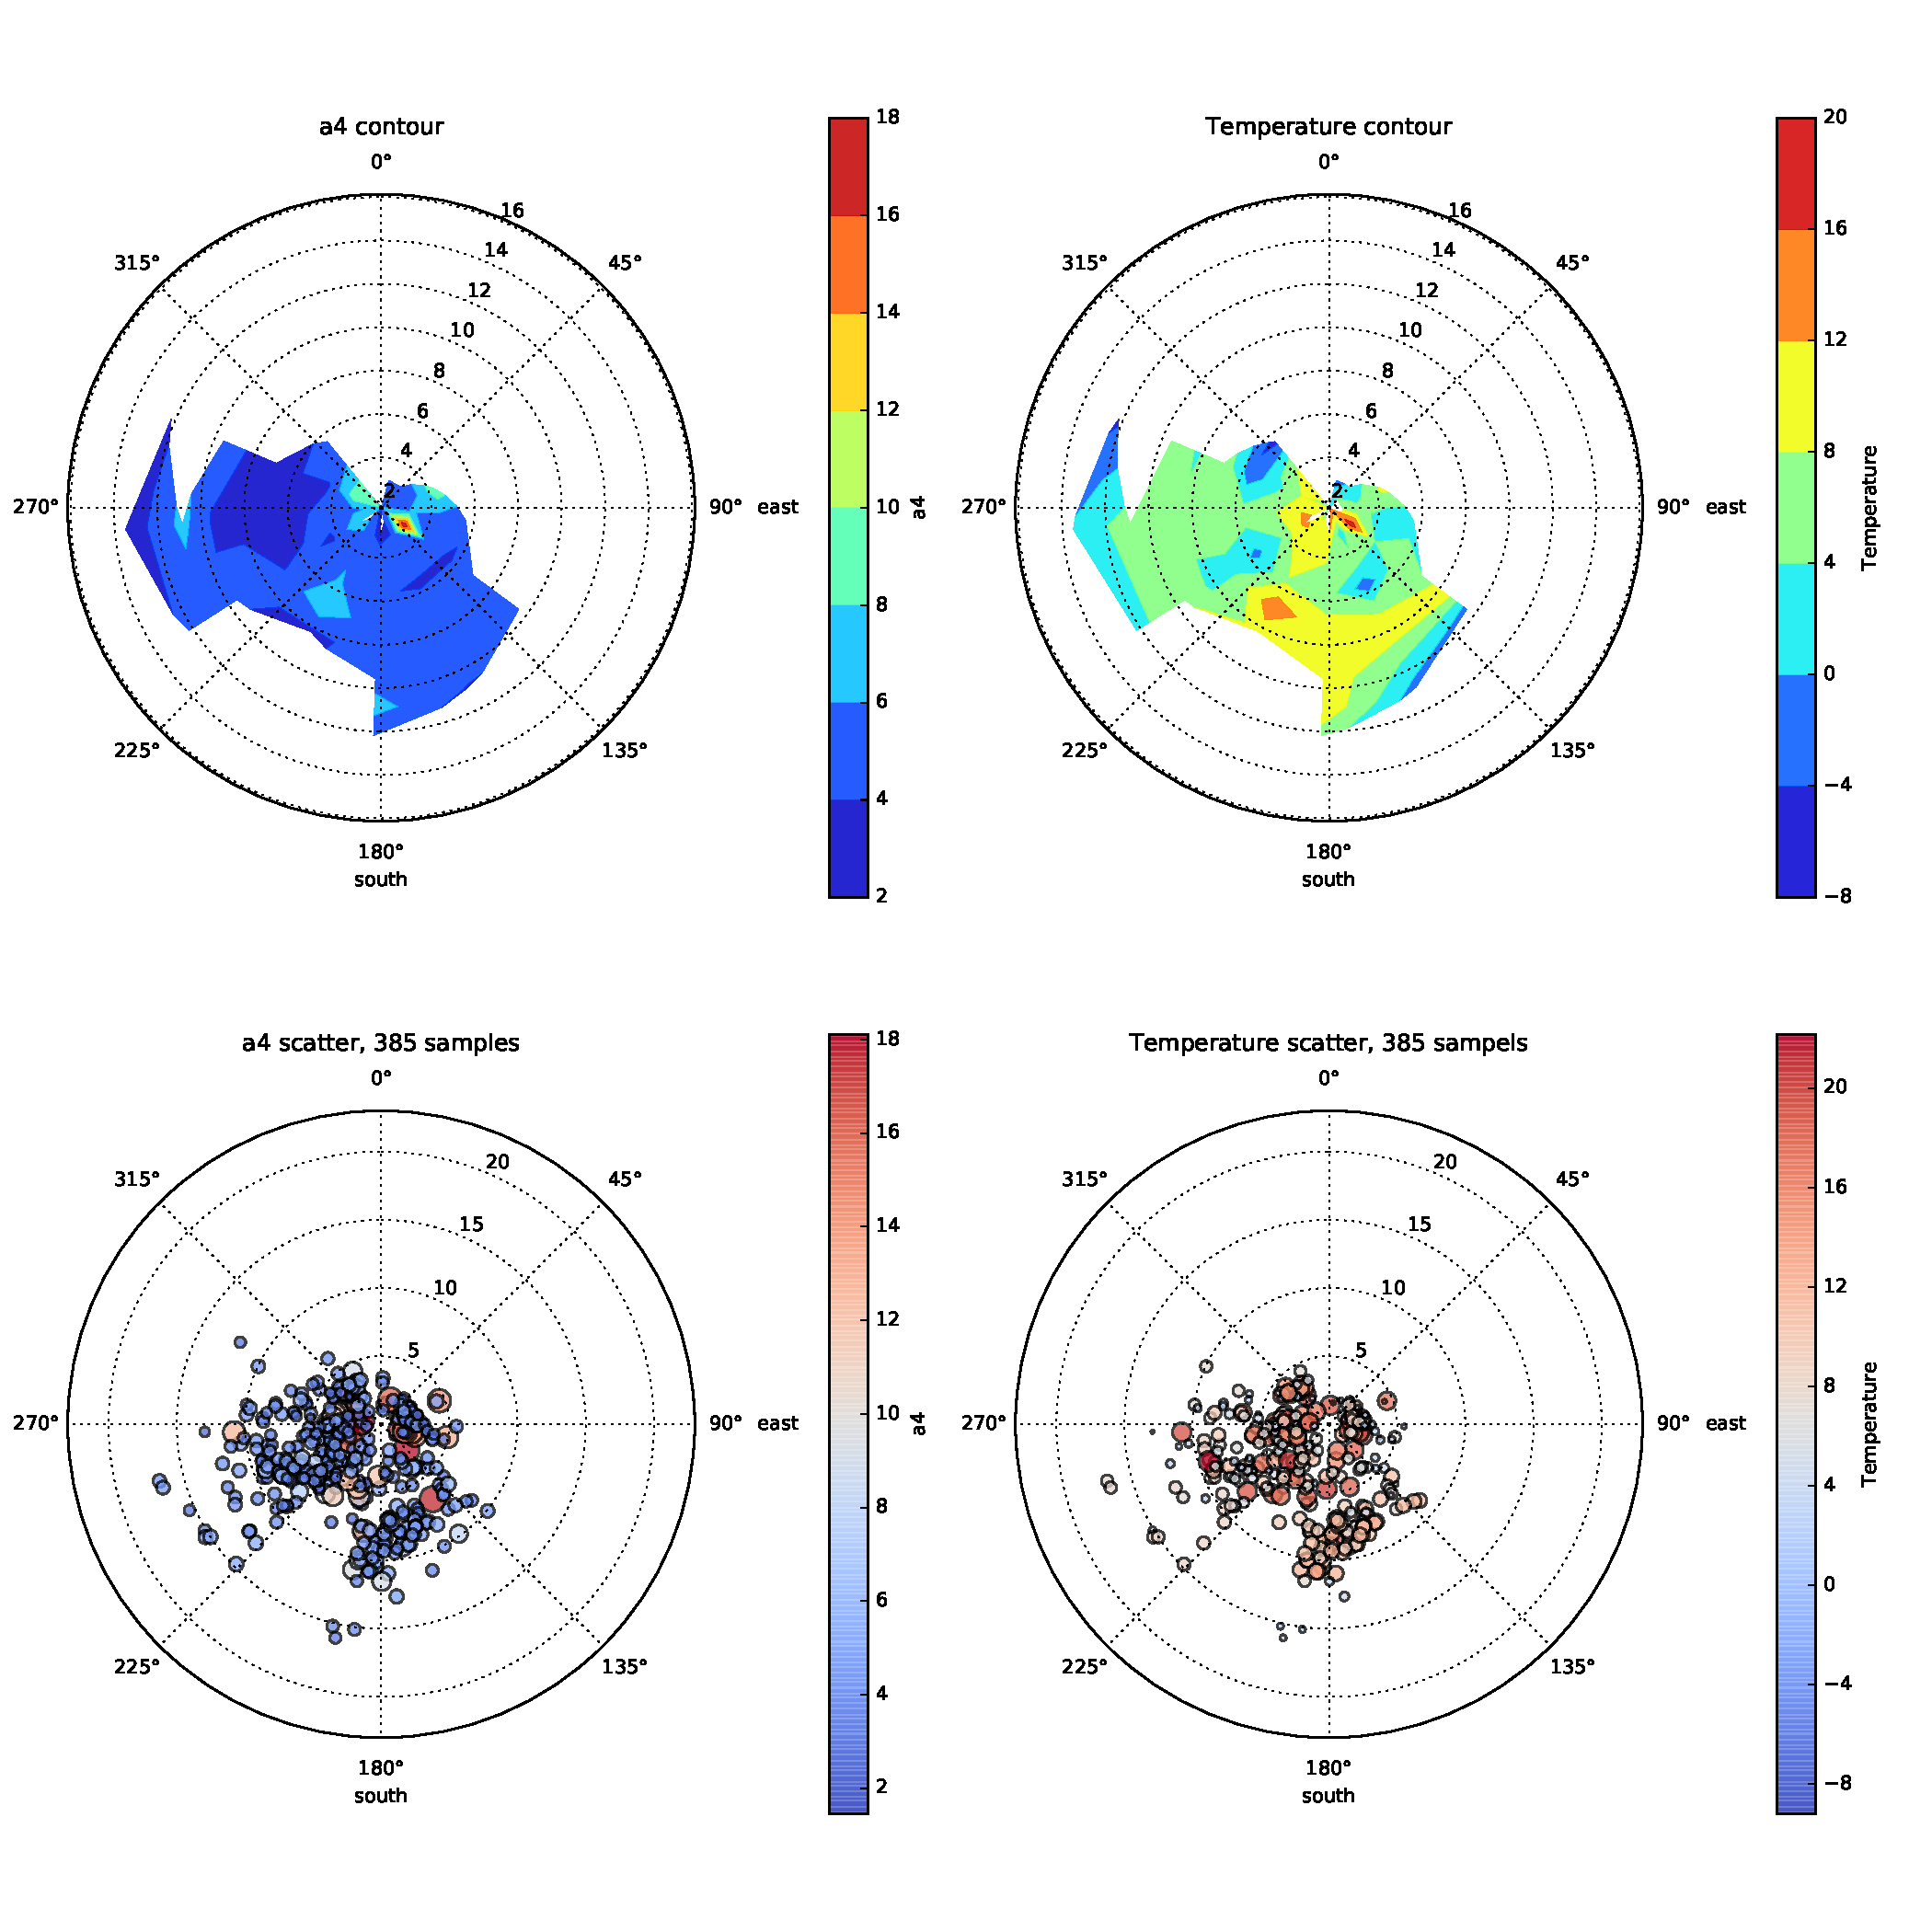
\includegraphics[scale=.46]{wind/wind_a4}
	\caption[Einfluss von Windgeschwindigkeit und Windrichtung auf $A_4$]{Einfluss von Windgeschwindigkeit und Windrichtung auf $A_4$. Die Plots in der linken Spalte zeigen $A_4$ gemäß der Farbskala an. Im unteren Plot ist die Größe der Kreise zusätzlich proportional zu $A_4$. Jeder Kreis repräsentiert eine von 385 Fokusaufnahmen. Analog stellt die rechte Spalte die Temperatur dar. Die Position in Polarkoordinaten wird durch den Wind bestimmt. Der Winkel entspricht der Windrichtung, der Abstand vom Nullpunkt entspricht der Windstärke in \si{\metre\per\second}.}
    \label{wind_a4_inline}
\end{figure}
\pagebreak

Ein Blick auf den Streuplot und den daraus hergeleiteten Flächeninterpolanten macht deutlich, dass die Sekundärspiegelposition und somit der Fokus in erster Linie temperatur- aber auch elevationsabhängig ist (Abb. \ref{foc_med_inline}). Jedoch sind die Isolinien nicht streng linear. Der Fokus in Abhängigkeit der Elevation ist bis zu einem Wert von $\sim\num{.7}$ nahezu konstant und steigt dann näherungsweise linear an. Dieses Verhalten tritt allerdings nur an den Temperaturgrenzbereichen aus. Bei mittleren Temperaturen, verhält sich der Fokus in Abhängigkeit der Elevation nahezu konstant. In Abhängigkeit von der Temperatur verhält sich der Fokus stark linear, zeigt jedoch auch hier leichte Abweichungen: im mittleren Temperaturbereich besteht ein Plateau etwas geringerer Steigung.\\

\begin{figure}[H]
	\centering
	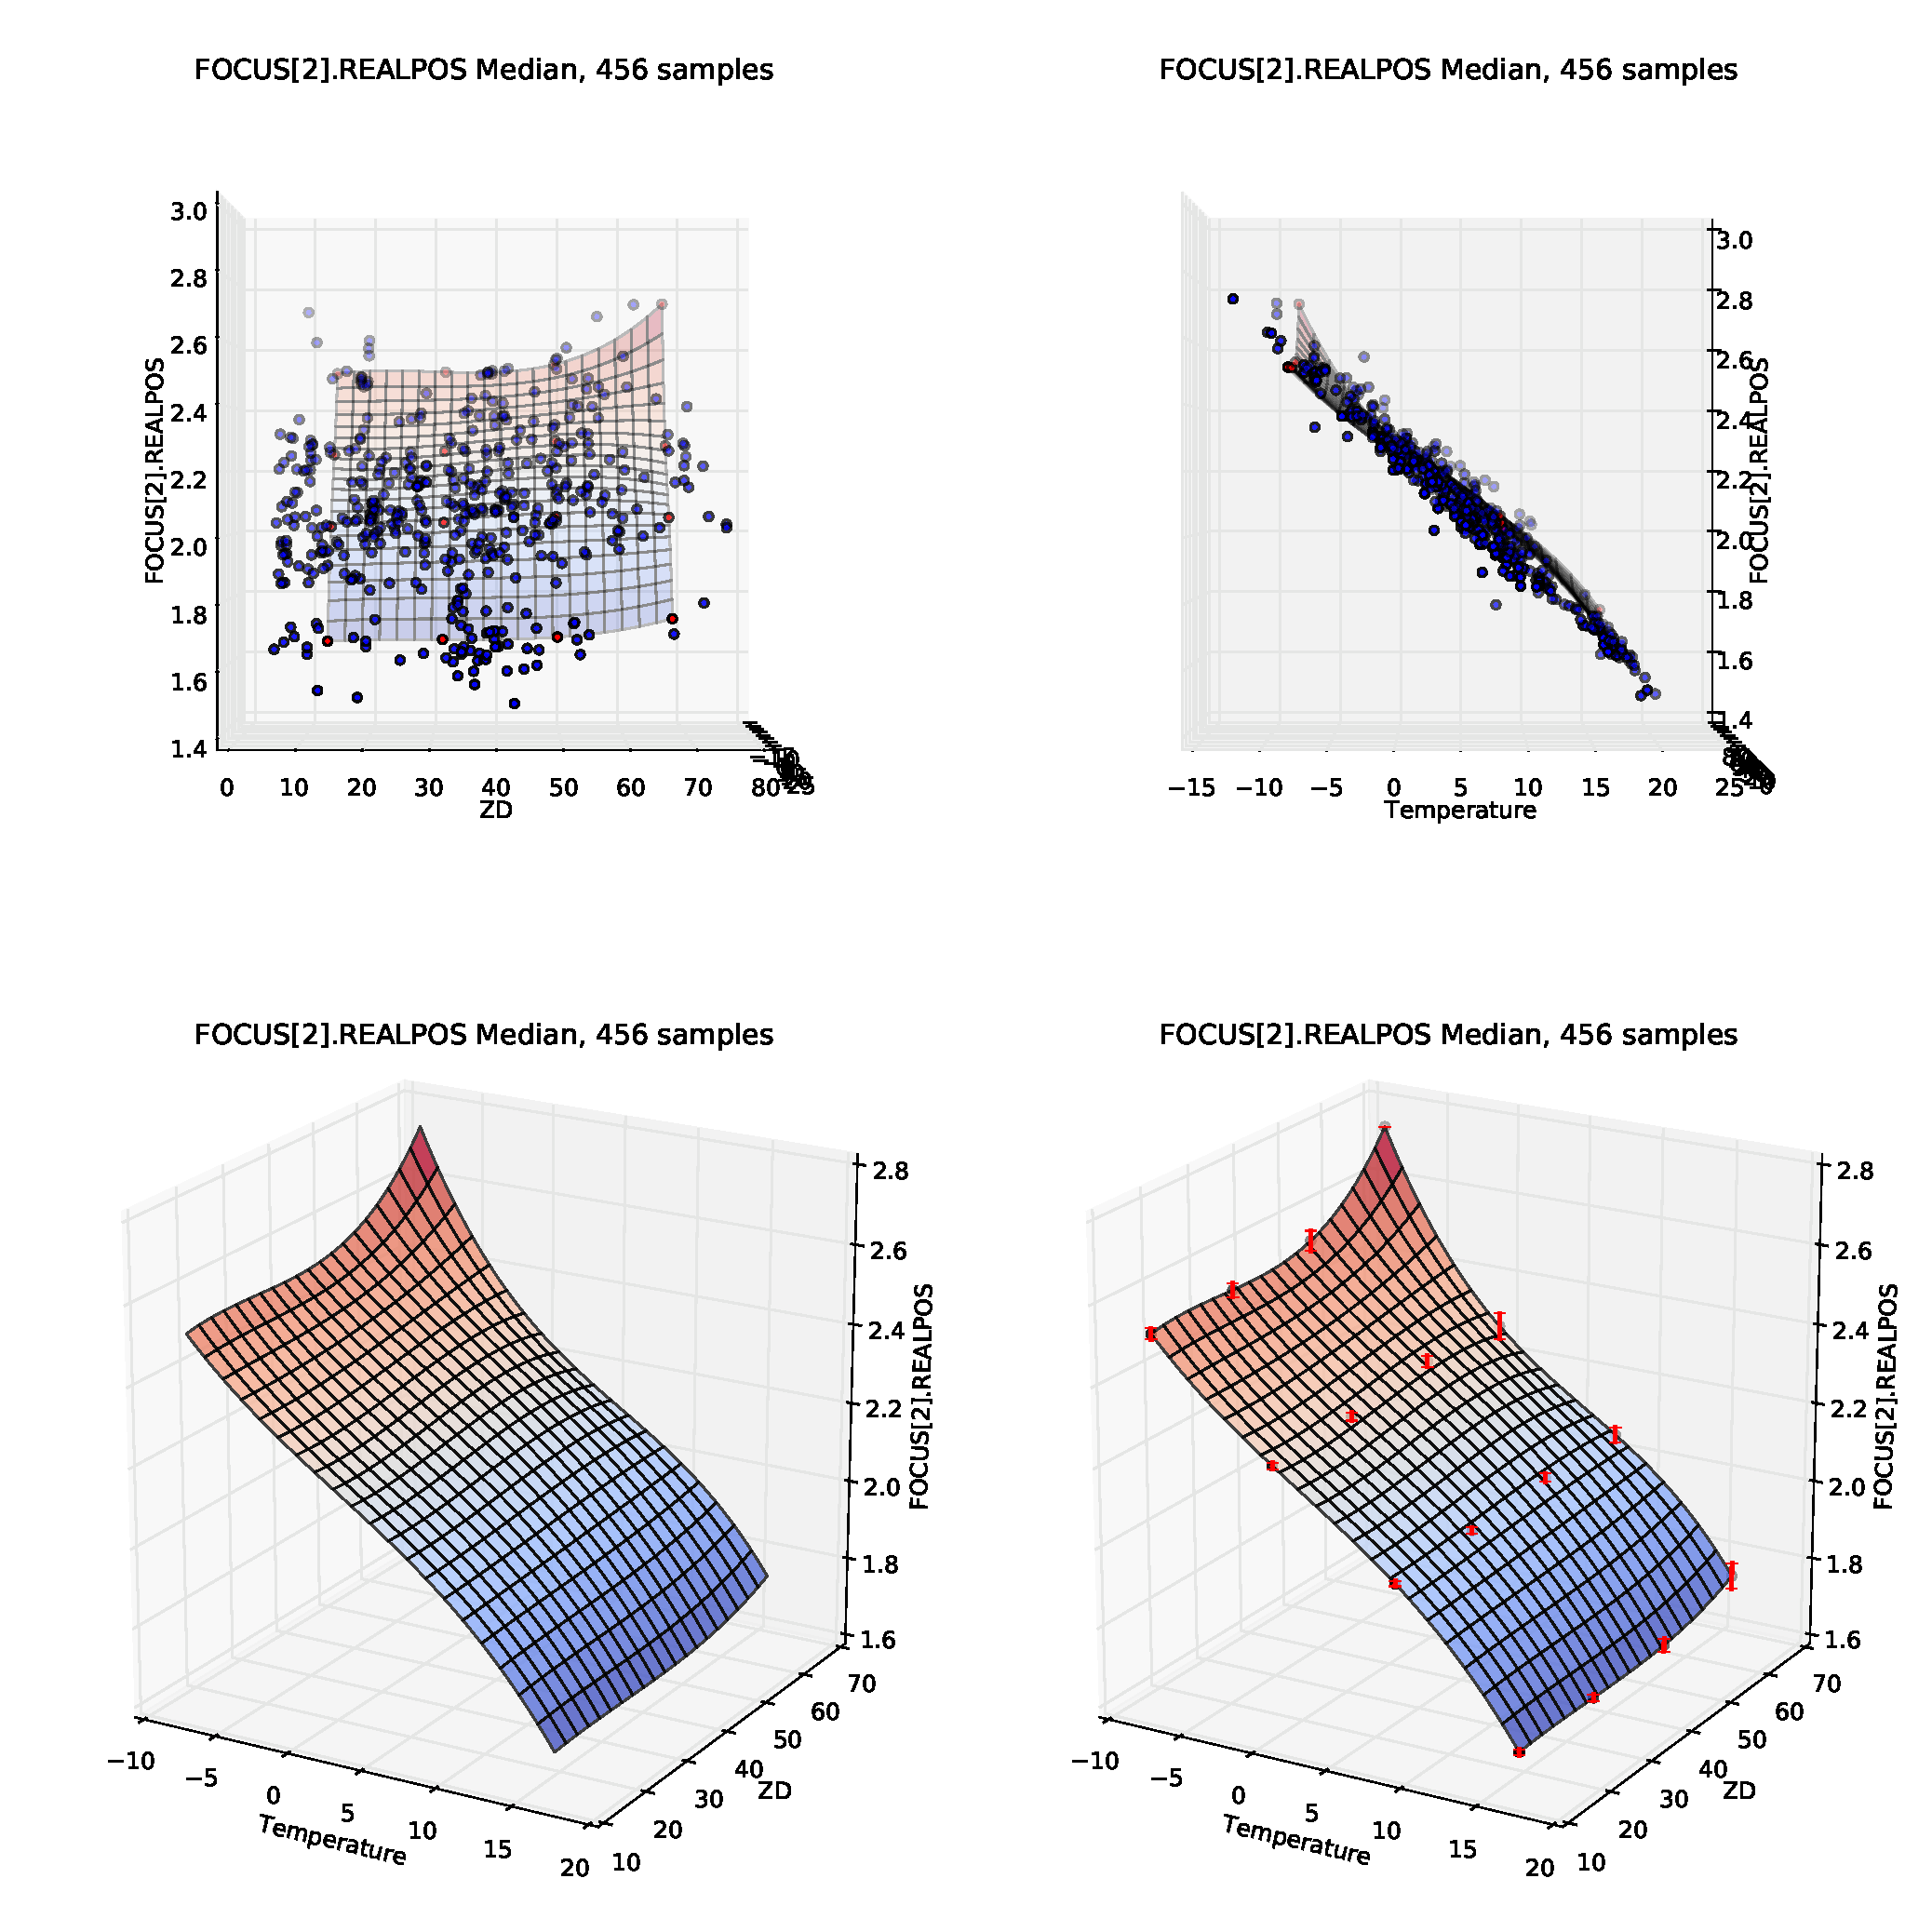
\includegraphics[scale=.44]{tsi_surf/POSITION_INSTRUMENTAL_FOCUS_2__REALPOS_med.pdf}
 	\caption[Temperatur- und Elevationsabhängigkeit der Sekundärspiegelposition]{Temperatur- und Elevationsabhängigkeit der Sekundärspiegelposition entlang der optischen Achse. Die Sekundärspiegelposition von 456 Fokusaufnahmen entsprechen den blauen Punkten. Die roten Kontrollpunkte im Plot unten rechts wurden über den Median aller Punkte in ihrer Umgebung gebildet und enthalten einen roten Fehlerbalken.}
    \label{foc_med_inline}
\end{figure}

Da die Streuung des Fokus in Form von Standardvariation als auch Varianz im Temperatur/Elevations-Raum für die besten Aufnahmen einer Fokusserie mit Werten von $\le\SI{5.0}{\percent}$ nur sehr gering ausfällt (Abb. \ref{psf_surf_a4_std_inline} und \ref{psf_surf_a4_var_inline}), ist der auf den Median-Kontrollpunkten basierende Interpolant der temperatur- und elevationsabhängigen Sekundärspiegelposition ein guter Kandidat für eine präzisere Fokusfunktion. Die B-Spline Fläche wurde als alleinstehendes Python-Skript ausgekoppelt, um in das Teleskop-System eingebunden zu werden (siehe \ref{focus.py}).

\begin{figure}[H]
	\centering
	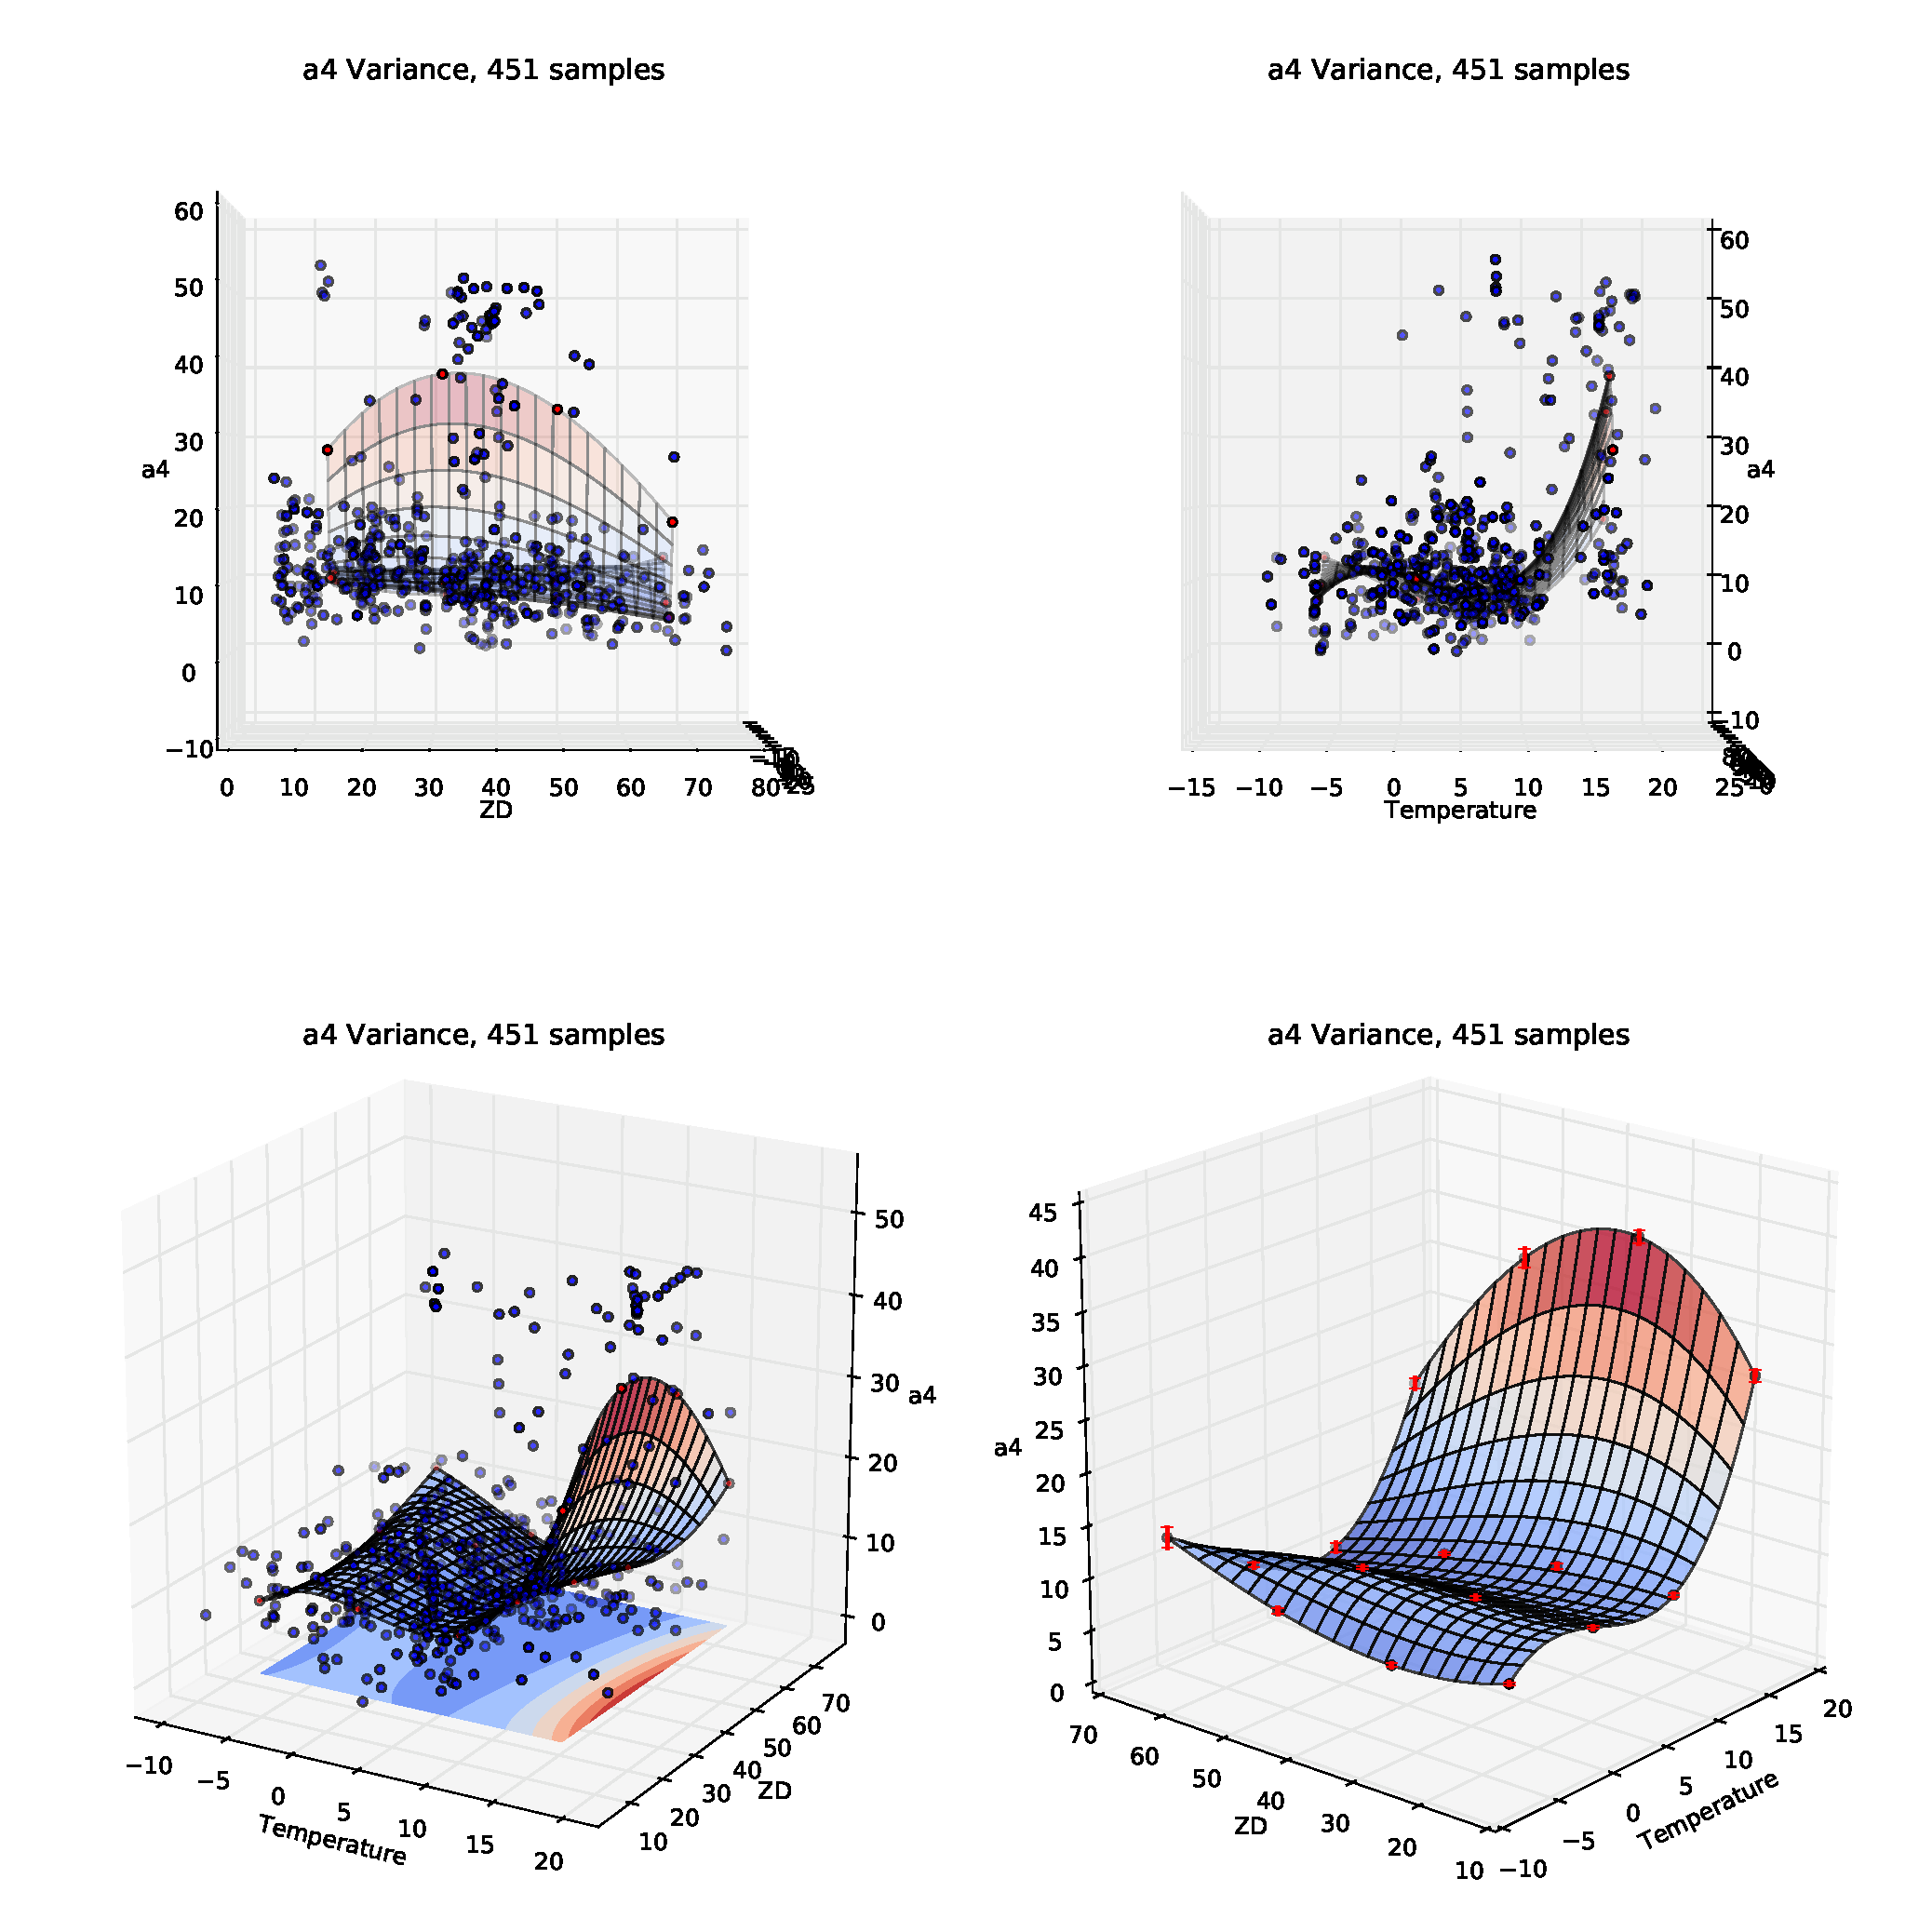
\includegraphics[scale=.48]{psf_surf/a4_var.pdf}
	\caption[Varianz Temperatur- und Elevationsabhängigkeit von $A_4$]{Varianz Temperatur- und Elevationsabhängigkeit von $A_4$. Es liegen 451 Fokusaufnahmen zugrunde, die jeweils einem blauen Punkt entsprechen. Die Plots oben links und rechts entsprechen der Projektion auf die Temperatur- und Elevations-Achse respektive. Die roten Kontrollpunkt wurden als Durchschnittswerte berechnet (mean). Die roten Balken an den Kontrollpunkten im Plot unten rechts sind ein Maß für die Streuung des Kontrollpunktes. }
    \label{psf_surf_a4_var_inline}
\end{figure}

\section{Zukunftsaussicht}
Die in den Korrelationsmatrizen enthaltene Transinformation kann als ein erster Anhaltspunkt dienen, um weitere Abhängigkeiten der Fokusfunktion aufzudecken oder schädliche Effekte auf die Bildqualität aufzuspüren. Dazu gehört, dass unter Umständen auch auch höhere Momente der PSF-Parameter betrachtet werden und mit den weiteren Freiheitsgraden des Hexapod, der den Sekundärspiegel justiert, korrigiert werden.\\
In Hinblick auf den Defokus sollte aufgrund des geringen Fehlers der Interpolant genauere Ergebnisse als die linear genäherte Fokusfunktion liefern. Weitere Fokusserien, die im Verlauf der Zeit aufgenommen werden, können die Genauigkeit des Interpolanten sogar erhöhen. Der Idealfall wäre eine Fokusfunktion, die alle Abhängigkeiten berücksichtigt, die zu einem Driften des Fokus führen und diese automatisch in einem ersten Schritt korrigiert, so dass eine Serie von Fokusaufnahmen gar nicht mehr notwendig ist.
